\documentclass[11pt]{article}
\usepackage{rldm25}
\usepackage{palatino}
\usepackage{graphicx}
\usepackage{amsmath}
\usepackage[T1]{fontenc}
\usepackage{lmodern}  % Fuente moderna con soporte completo
\usepackage{hyperref}
\usepackage{array}
\usepackage{tabu}
\renewcommand{\bfdefault}{b} % Asegura que las negritas se activen
\usepackage{caption}
\captionsetup[table]{textfont={it}, labelfont={bf}, singlelinecheck=false, labelsep=newline}

% definitions for citeproc citations
\NewDocumentCommand\citeproctext{}{}
\NewDocumentCommand\citeproc{mm}{%
  \begingroup\def\citeproctext{#2}\cite{#1}\endgroup}
\makeatletter
 % allow citations to break across lines
 \let\@cite@ofmt\@firstofone
 % avoid brackets around text for \cite:
 \def\@biblabel#1{}
 \def\@cite#1#2{{#1\if@tempswa , #2\fi}}
\makeatother
\newlength{\cslhangindent}
\setlength{\cslhangindent}{1.5em}
\newlength{\csllabelwidth}
\setlength{\csllabelwidth}{3em}
\newenvironment{CSLReferences}[2] % #1 hanging-indent, #2 entry-spacing
 {\begin{list}{}{%
  \setlength{\itemindent}{0pt}
  \setlength{\leftmargin}{0pt}
  \setlength{\parsep}{0pt}
  % turn on hanging indent if param 1 is 1
  \ifodd #1
   \setlength{\leftmargin}{\cslhangindent}
   \setlength{\itemindent}{-1\cslhangindent}
  \fi
  % set entry spacing
  \setlength{\itemsep}{#2\baselineskip}}}
 {\end{list}}
\usepackage{calc}
\newcommand{\CSLBlock}[1]{\hfill\break\parbox[t]{\linewidth}{\strut\ignorespaces#1\strut}}
\newcommand{\CSLLeftMargin}[1]{\parbox[t]{\csllabelwidth}{\strut#1\strut}}
\newcommand{\CSLRightInline}[1]{\parbox[t]{\linewidth - \csllabelwidth}{\strut#1\strut}}
\newcommand{\CSLIndent}[1]{\hspace{\cslhangindent}#1}

\usepackage{longtable,booktabs,array}
\usepackage{calc} % for calculating minipage widths
% Correct order of tables after \paragraph or \subparagraph
\usepackage{etoolbox}
\makeatletter
\patchcmd\longtable{\par}{\if@noskipsec\mbox{}\fi\par}{}{}
\makeatother
% Allow footnotes in longtable head/foot
\IfFileExists{footnotehyper.sty}{\usepackage{footnotehyper}}{\usepackage{footnote}}
\makesavenoteenv{longtable}

\usepackage{graphicx}
\makeatletter
\newsavebox\pandoc@box
\newcommand*\pandocbounded[1]{% scales image to fit in text height/width
  \sbox\pandoc@box{#1}%
  \Gscale@div\@tempa{\textheight}{\dimexpr\ht\pandoc@box+\dp\pandoc@box\relax}%
  \Gscale@div\@tempb{\linewidth}{\wd\pandoc@box}%
  \ifdim\@tempb\p@<\@tempa\p@\let\@tempa\@tempb\fi% select the smaller of both
  \ifdim\@tempa\p@<\p@\scalebox{\@tempa}{\usebox\pandoc@box}%
  \else\usebox{\pandoc@box}%
  \fi%
}
% Set default figure placement to htbp
\def\fps@figure{htbp}
\makeatother

\title{Modelling Pavlovian Attentional Biases Using Reinforcement
Learning}

\author{
  Francisco Garre-Frutos\thanks{Mind, Brain and Behavior Research Center
(CIMCYC) and Department of Experimental Psychology, University of
Granada, Granada, Spain}\\
            University of Granada \\ % Nombre de la afiliación
              Granada, Spain \\ % Dirección de la afiliación
                  \texttt{fgfrutos@ugr.es} \\ % Email
        \And % Salto estándar
    David Luque\thanks{Department of Basic Psychology and Málaga
Institute of Biomedical Research (IBIMA), University of Málaga, Málaga,
Spain}\\
            University of Malaga \\ % Nombre de la afiliación
              Málaga, Spain \\ % Dirección de la afiliación
                  \texttt{dluque@uma.es} \\ % Email
        \AND % Salto de columna si "note" está presente
    Pablo Martínez-López\footnote[2]\\\\
            University of Malaga \\ % Nombre de la afiliación
              Málaga, Spain \\ % Dirección de la afiliación
                  \texttt{mlpablocorreo@gmail.com} \\ % Email
        \And % Salto estándar
    Juan Lupiáñez\footnote[1]\\\\
            University of Granada \\ % Nombre de la afiliación
              Granada, Spain \\ % Dirección de la afiliación
                  \texttt{jlupiane@ugr.es} \\ % Email
        \And % Salto estándar
    Miguel A. Vadillo\thanks{Department of Basic Psychology, Autonomous
University of Madrid, Madrid, Spain}\\
            Autonomous University of Madrid \\ % Nombre de la afiliación
              Madrid, Spain \\ % Dirección de la afiliación
                  \texttt{miguel.vadillo@uam.es} \\ % Email
      % No añadir nada si es el último autor
  }



\begin{document}

\AtBeginEnvironment{table}{\setlength\belowcaptionskip{0pt}}

\maketitle

\begin{abstract}
A central question in modern models of Pavlovian learning is how
learning influences attention. Mackintosh's theory proposes that stimuli
that reliably predict significant outcomes receive more attention to
maximize learning, whereas Pearce-Hall's theory proposes that
uncertainty drives attention to promote exploration. Empirical evidence
supports both views, showing that stimuli that consistently predict
reward or reward variability are more likely to capture attention, even
when they act as distractors in conflict with other goal-relevant
stimuli. Although these findings are often assumed to reflect the
mechanisms of Mackintosh and Pearce-Hall, there have been surprisingly
few attempts to explicitly model the learning dynamics underlying such
attentional biases. In this work, we developed two hierarchical Bayesian
models implementing Mackintosh and Pearce-Hall principles and compared
their fit to two datasets in which either value or uncertainty was
manipulated. Surprisingly, our results show that the Pearce-Hall model
can account for both experimental effects. We argue that this likely
reflects a methodological confound in how value is typically
manipulated, as high-value cues often also exhibit greater outcome
variance, raising the possibility that some experimental effects reflect
uncertainty-driven rather than value-driven attention.
\end{abstract}

\keywords{reinforcement
learning, Pavlovian, value, uncertainty, attention }

\acknowledgements{This work was supported by an FPU predoctoral grant
(ref. FPU20/00826) to FGF.}  

\startmain % to start the main 1-4 pages of the submission.

\section{Introduction}\label{introduction}

The relationship between learning and attention has been a central
question in Pavlovian learning for decades. Since Rescorla \& Wagner
(1972), numerous accounts have attempted to incorporate attention into
associative learning models. For example, Mackintosh (1975) proposed
that attention increases for cues that reliably predict significant
outcomes, thereby promoting further learning about those cues, whereas
Pearce \& Hall (1980) argued that attention increases for cues
associated with greater uncertainty or variability in outcomes, thereby
promoting exploratory learning. Both principle have received empirical
support. For instance, in the study by Le Pelley et al. (2015),
participants performed a visual search task in which singleton
distractors were consistently paired with two different reward
magnitudes. In this procedure, although the distractors predicted
reward, looking directly at them caused omission of reward, even though
attending to the high-reward predictive distractor was counterproductive
to the task goals, Le Pelley et al. (2015) found that participants
tended to look more at high than the low-value distractor, reflecting a
Pavlovian bias that contradicted the participants' goals.

According to Le Pelley et al. (2016), this attentional bias could be
explained by a modified Mackintosh model, in which the associative
strength (\(V\)) of a distractor is described by the following
Rescorla-Wagner rule: \begin{equation}\phantomsection\label{eq-1}{ 
V_{n} = V_{n-1} + \eta\,\alpha_{n}\,\bigl(\lambda_{n} - V_{n-1}\bigr)
}\end{equation} where \(\eta\) is a learning rate parameter, \(\lambda\)
is the reward in trial \(n\), and \(\alpha\) is a weight parameter
reflecting attention to the cue. From this formula, \(V_{n}\) is updated
as a function of the prediction error,
\(\bigl(\lambda_{n} - V_{n-1}\bigr)\). Unlike other formulations of the
Mackintosh model, Le Pelley et al. (2016) assumed that \(\alpha\) is
updated as \begin{equation}\phantomsection\label{eq-2}{
\alpha_{n} = \lvert V_{n-1}\rvert
}\end{equation} In other words, attention to the cue is a function of
the asymptotic \(\lambda\). This formulation of the Mackintosh model can
explain why value-driven distraction increases over trials and remains
stable with training.

In contrast, Pearce et al. (1982) postulated that attention is mainly
driven by prediction errors:
\begin{equation}\phantomsection\label{eq-3}{
\alpha_{n} = \gamma\,\lvert \lambda_{n} - V_{n-1}\rvert 
+ \bigl(1 - \gamma\bigr)\,\alpha_{n-1}
}\end{equation} where \(\gamma\) is a decay parameter that weights the
relevance of previous values of \(\alpha\). The Pearce-Hall principle
predicts that cues associated with more variable outcomes (and thus
higher prediction errors) will receive more attention. Consistent with
this prediction, and using a procedure similar to Le Pelley et
al.~(2015), Pearson et al. (2024) showed that when irrelevant
distractors were associated with different levels of reward variability,
high-variance distractors received more attention than low-variance
distractors, even when the overall expected value was higher for
low-variance distractors (see also Le Pelley et al., 2019).

The results of both Le Pelley et al.~(2015) and Pearson et al. (2024)
suggest that the principles of Mackintosh and Pearce-Hall may be
applicable in different contexts. Despite explicit formulations of how
attention should change as a function of learning, there are few
attempts to explicitly model the learning dynamics associated with
either theory in Pavlovian attentional biases. In light of this, in this
work, we developed two hierarchical Bayesian reinforcement learning (RL)
models in which attention is modeled according to formulas (2) and (3).
We then fit these two models to two openly aviable datasets where either
reward value or uncertainty is manipulated, and compared the peformance
of each model to describe the data.

\section{Method}\label{method}

\subsection{Data}\label{data}

We used the open-source data from Experiment 2 of the Le et al. (2024)
study and Experiment 1 of the Chow et al. (2024) study. In both
experiments, participants performed the additional singleton task
(Theeuwes, 1992). In each trial, participants had to search for unique
diamond-shaped stimulus surrounded by circle non-target shapes, one of
which was a color-singleton distractor (a circle of a different color)
(Figure 1). Critically, during the task, participants could earn rewards
(points) depending on the color of the distractor. In the Le et al.
(2024) study, if participants managed to look at the target stimuli
without looking at the distractor, they would earn either a high or low
reward depending on the color of the distractor (a high-reward or a
low-reward color). However, looking at the distractor would result in
the omission of the reward. In Chow et al. (2024), the color of the
distractor signaled outcome variability. One distractor color was always
associated with the same outcome (low variance), while the other
singleton distractor signaled two possible outcomes (high variance) with
a 50\% probability. The expected value of both distractors, however, was
matched overall.

\begin{figure}

\centering{

\pandocbounded{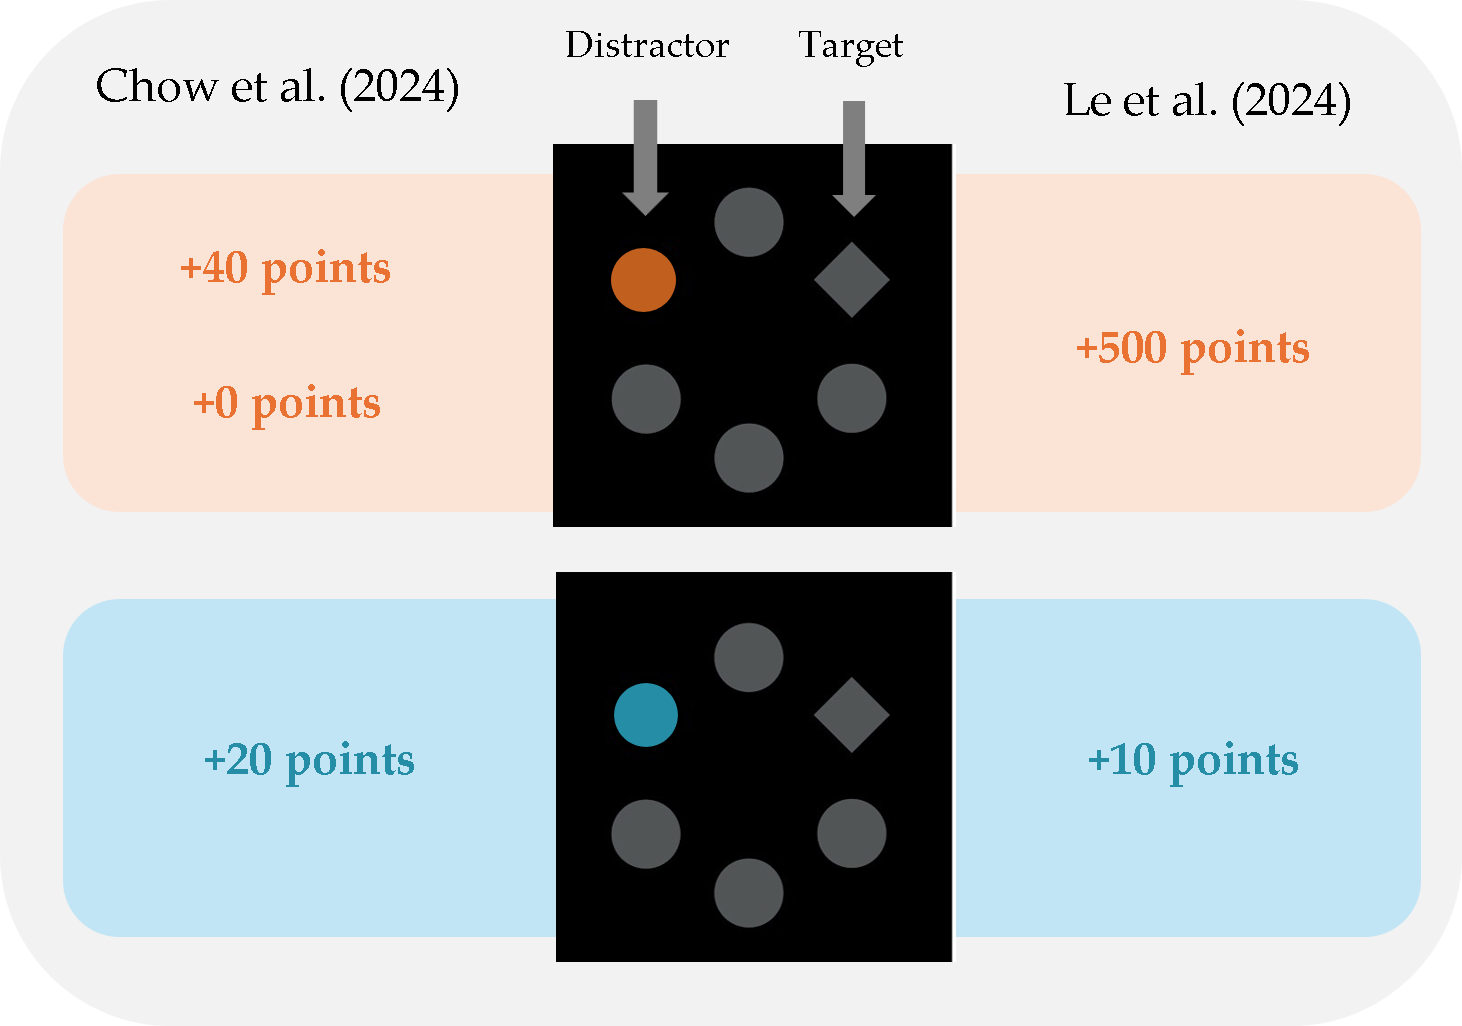
\includegraphics[keepaspectratio]{Output/figures/figure_1.png}}

}

\caption{\label{fig-1}Schematic representation of the task design. In Le
et al.~(2024), the high-value distractor (top) was associated with more
reward than the low-value distractor (bottom), although looking at the
distractor before the target produced reward omission. In Chow et
al.~(2024), the high-variance distractor was associated with two
possible outcomes at 50\% probability, while the low-variance distractor
was always associated with the same outcome.}

\end{figure}%

We employed this two specific datasets because they are directly
comparable in design and have an unusually large number of participants
compared to much of the literature. In Experiment 2 of Le et al. (2024),
there are 84 participants with 384 trials each, whereas in Chow et al.
(2024), there are 40 participants with 512 trials each. We provide the
data and analysis code for this study in the following repository:
\url{https://github.com/franfrutos/rldm25_vmac}.

\subsection{Model Specification}\label{model-specification}

For the datasets described above, we model whether a participant looked
at the distractor (1) or the target (0) on trial \(i\). This is
implemented using a logistic regression (\(\text{logit}^{-1}\)
function), where \(\operatorname{Pr}(\text{Look}_{i} = 1)\) is
determined by the latent attention (\(\alpha\)) for each distractor
(\(s\)): \begin{equation}\phantomsection\label{eq-4}{
\begin{aligned}
\operatorname{Pr}(\text{Look}_{i} = 1) \sim \text{Bernoulli}(\theta_{i}),\\
\theta_{i} = \frac{1}{1 + e^{-(\beta_{0,j} + \beta_{1,j} \cdot \alpha_{s[i]} + \beta_{2,j} \cdot t_{i})}},
\end{aligned}
}\end{equation} where \(\beta_{0,j}\) is the intercept for subject
\(j\), \(\beta_{1,j}\) is the slope that relates \(\alpha\) to the
probability of looking at the distractor, and \(\beta_{2,j}\) controls
for practice effects across trials (\(t\)). This simple logistic
function can be viewed as a softmax rule with two levels: the target
(reference) and the distractor. Thus, \(\beta_{0}\) can be interpreted
as a bias term (a tendency to choose the target or the distractor), and
\(\beta_{1}\) as an \emph{inverse temperature} parameter. We
parameterized \(\beta_{1}\) as \(\text{logit}^{-1}(\cdot)\cdot 10\), so
it could only take positive values in the range {[}0, 10{]}. A higher
\(\beta_{1}\) increases selection of distractors with higher \(\alpha\).

On trial \(i\), each distractor \(s\) updates its \(V_{s}\) according to
equation (1), where \(\lambda_{i}\) equals the observed
reward\footnote{\(\lambda\) is scaled by
  \(\frac{\lambda_{i}}{\max(\lambda)}\), which ensures that \(V\) takes
  values in the range {[}0, 1{]}.} on that trial. Regarding
\(\alpha_{s}\), both models assume that participants start with an
initial level of attention (\(\alpha_0\)). Then, in the
\emph{Mackintosh} model (Le Pelley et al., 2016), \(\alpha\) is updated
according to equation (2), while in the \emph{Pearce-Hall} model,
\(\alpha\) is updated following equation (3), where \(\eta\) and
\(\gamma\) are subject-specific parameters governing the update of \(V\)
and \(\alpha\).

All subject-specific parameters (\(k\)) are assumed to be drawn from a
normal distribution, using non-centered parameterization to improve
sampling efficiency: \begin{equation}\phantomsection\label{eq-5}{
\beta_{k,j} = \mu_{k} + \sigma_{k} \cdot z_{k,j}, \quad z_{k,j} \sim \mathcal{N}(0, 1).
}\end{equation} Subject-specific parameters (\(\beta_{k,j}\)) are
modeled by scaling group-level means (\(\mu_{k}\)) with individual
deviations (\(\sigma_k\)) and standardized parameters (\(z_{k,j}\)).
Bounded parameters (\(\eta\), \(\gamma\), \(\alpha_{0}\), and
\(\beta_{1}\)) are then transformed using the \(\text{logit}^{-1}\)
function to ensure they remain within the {[}0, 1{]} interval. We used
weakly informative priors (\(\mathcal{N}(0, 1)\)) for group-level means
\(\mu\), and truncated normals for \(\sigma\).

\section{Results}\label{results}

The models described above were programmed in Stan (Stan Development
Team, 2024). We fit both models to each dataset using 6000 warm-up
iterations and 8000 samples across four chains (\(\bar{R} < 1.01\)). We
assessed the relative fit of the two models to each dataset using the
Pareto-smoothed importance sampling leave-one-out cross-validation
(PSIS-LOO; Vehtari et al., 2017). Table 1 shows the relative performance
of the \emph{Mackintosh} model compared to the \emph{Pearce-Hall} model,
where a negative ELPD means worse performance.

\begin{table}[!h]
\centering
\caption{\label{tab:unnamed-chunk-3}Relative fit analysis}
\centering
\fontsize{10}{12}\selectfont
\begin{tabu} to \linewidth {>{\raggedright}X>{\centering}X>{\centering}X>{\centering}X>{\centering}X}
\toprule
\multicolumn{1}{c}{ } & \multicolumn{2}{c}{Chow et al. (2024)} & \multicolumn{2}{c}{Le et al. (2024)} \\
\cmidrule(l{3pt}r{3pt}){2-3} \cmidrule(l{3pt}r{3pt}){4-5}
Model & $\Delta$ELPD & $\Delta$SE & $\Delta$ELPD & $\Delta$SE\\
\addlinespace
\midrule
Pearce-Hall & 0 & 0 & 0 & 0\\
Mackintosh & -254 & 24 & -79 & 21\\
\bottomrule
\multicolumn{5}{l}{\rule{0pt}{1em}\textit{Note.} ELPD = Expected Log-Pointwise Predictive Density. SE = Standard Error.}\\
\end{tabu}
\end{table}

According to Vehtari et al. (2017), if the difference in ELPD between
models deviates by more than 2 SEs, the model with the higher ELPD is
likely to be the better fit for the data. By this criterion, the
\emph{Pearce-Hall} model outperformed the \emph{Mackintosh} model in
both datasets.

\begin{figure}

\centering{

\pandocbounded{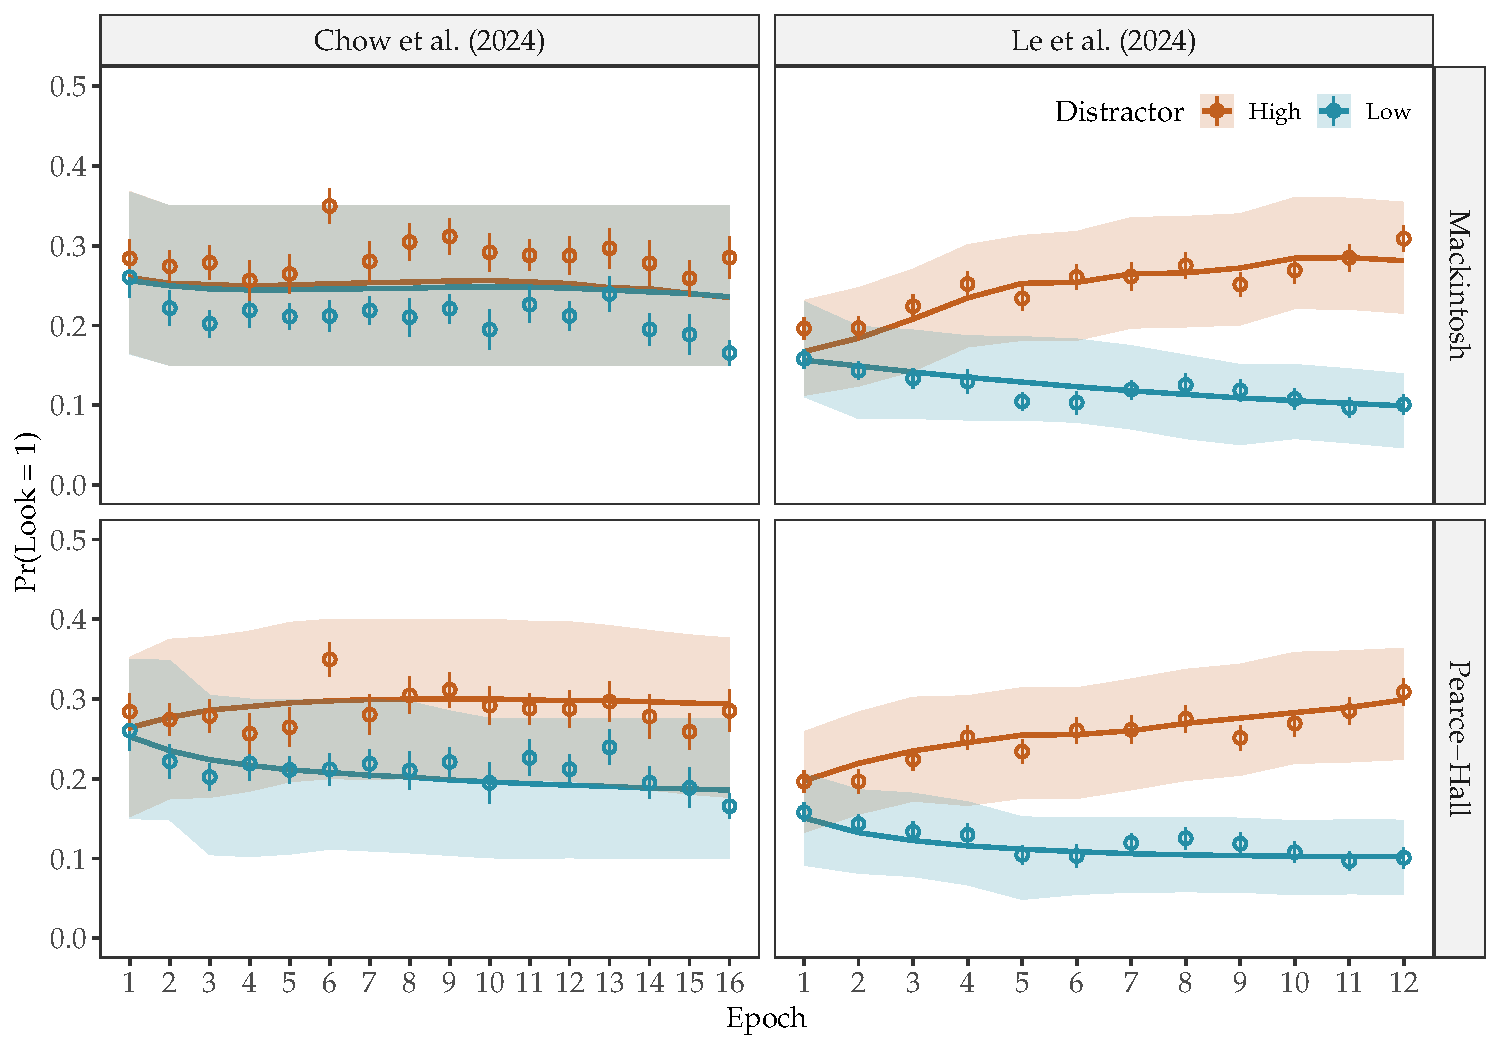
\includegraphics[keepaspectratio]{rldm25_vmac_abstract_files/figure-pdf/fig-2-1.pdf}}

}

\caption{\label{fig-2}Posterior Predictive Checks (PPC) for the
\emph{Mackintosh} and \emph{Pearce-Hall} models, split by dataset. PPCs
were generated by simulating new observations based on the fitted
parameters and aggregating results at the group level. Solid lines
represent the mean, and the shaded area is the 89\% High Density
Interval (HDI) of the posterior predictions across epochs of 32 trials.
The dots represent the observed mean proportion of gazes at the
distractor, while the error bars show the SEM.}

\end{figure}%

Although the previous analysis suggests that \emph{Pearce-Hall} has the
best relative fit for Le et al. (2024) and Chow et al. (2024) datasets,
we should also verify whether both models predict the theoretically
relevant experimental effects---namely, whether participants look more
often at the high-value (or high-variance) distractor relative to the
low-value (or low-variance) distractor. To examine this, we compared the
absolute fit of the \emph{Mackintosh} and \emph{Pearce-Hall} models via
Posterior Predictive Checks (PPC). Figure 2 displays the PPCs as a
function of distractor type and epochs (32-trial bins). As expected, the
\emph{Pearce-Hall} model alone captures the greater attention to the
high-variance distractor in the Chow et al. (2024) dataset, whereas the
\emph{Mackintosh} model predicts no differences between distractors,
because the asymptotic \(\lambda\) was matched. Interestingly, although
the \emph{Mackintosh} model provides a reasonable fit to Le et al.
(2024) data, the \emph{Pearce-Hall} model's predictions are closer. It
also appears to better capture the earlier stages of learning, which may
explain why it provides superior predictive accuracy.

\section{Conclusions}\label{conclusions}

Our results show that it is possible to use RL models to capture
Pavlovian attentional biases. We found that when uncertainty is
manipulated (Chow et al., 2024), only the \emph{Pearce-Hall} model
explains the observed data. When value is manipulated (Le et al., 2024),
somewhat unexpectedly, \emph{Pearce-Hall} also predicts greater
attention to the high-value distractor. As suggested by Pearson et
al.~(2024), outcome variance is a measure of uncertainty because it
reflects the amount of prediction error associated with a cue. While
outcome variance is explicitly manipulated in Pearson et al. (2024), in
the paradigm used by Le Pelley et al. (2015), manipulation of value can
be confounded with differences in outcome variance between distractors.
As explained above, in Le Pelley et al. (2015), when participants look
at the distractors, they cause a reward omission, which can be viewed as
a prediction error. This prediction error is larger for the high-value
distractor than for the low-value distractor, and the proportion of
prediction errors increases as a function of attention because the
probability of looking at a distractor increases across trials only for
the high-value distractor. Thus, the high-value distractor not only
represents the highest value, but is also associated with greater
variability. This methodological confound may explain why the
\emph{Pearce-Hall} principle is a better fit for Le et al. (2024).

\section{References}\label{references}

\phantomsection\label{refs}
\begin{CSLReferences}{1}{0}
\bibitem[\citeproctext]{ref-chow2024}
Chow, J. Y. L., Garner, K. G., Pearson, D., Heber, J., \& Le Pelley, M.
E. (2024). Effects of instructed and experienced uncertainty on
attentional priority. \emph{Journal of Experimental Psychology:
Learning, Memory, and Cognition}.
\url{https://doi.org/10.1037/xlm0001427}

\bibitem[\citeproctext]{ref-le2024}
Le, J. T., Watson, P., \& Le Pelley, M. E. (2024). Effects of outcome
revaluation on attentional prioritisation of reward-related stimuli.
\emph{Quarterly Journal of Experimental Psychology}, 17470218241236711.
\url{https://doi.org/10.1177/17470218241236711}

\bibitem[\citeproctext]{ref-lepelley2016}
Le Pelley, M. E., Mitchell, C. J., Beesley, T., George, D. N., \& Wills,
A. J. (2016). Attention and associative learning in humans: An
integrative review. \emph{Psychological Bulletin}, \emph{142}(10),
11111140. \url{https://doi.org/10.1037/bul0000064}

\bibitem[\citeproctext]{ref-lepelley2015}
Le Pelley, M. E., Pearson, D., Griffiths, O., \& Beesley, T. (2015).
When Goals Conflict With Values: Counterproductive Attentional and
Oculomotor Capture by Reward-Related Stimuli. \emph{Journal of
Experimental Psychology: General}, \emph{144}, 158--171.
\url{https://doi.org/10.1037/xge0000037}

\bibitem[\citeproctext]{ref-lepelley2019}
Le Pelley, M. E., Pearson, D., Porter, A., Yee, H., \& Luque, D. (2019).
Oculomotor capture is influenced by expected reward value but (maybe)
not predictiveness. \emph{Quarterly Journal of Experimental Psychology},
\emph{72}(2), 168--181.
\url{https://doi.org/10.1080/17470218.2017.1313874}

\bibitem[\citeproctext]{ref-mackintosh1975}
Mackintosh, N. J. (1975). A theory of attention: Variations in the
associability of stimuli with reinforcement. \emph{Psychological
Review}, \emph{82}(4), 276--298. \url{https://doi.org/10.1037/h0076778}

\bibitem[\citeproctext]{ref-pearce1980}
Pearce, J. M., \& Hall, G. (1980). A model for pavlovian learning:
Variations in the effectiveness of conditioned but not of unconditioned
stimuli. \emph{Psychological Review}, \emph{87}(6), 532--552.
\url{https://doi.org/10.1037/0033-295X.87.6.532}

\bibitem[\citeproctext]{ref-pearce1982}
Pearce, J. M., Kaye, H., \& Hall, G. (1982). Predictive accuracy and
stimulus associability: Development of a model for pavlovian learning.
\emph{Quantitative Analyses of Behavior}, \emph{3}, 241--255.

\bibitem[\citeproctext]{ref-pearson2024}
Pearson, D., Chong, A., Chow, J. Y. L., Garner, K. G., Theeuwes, J., \&
Le Pelley, M. E. (2024). Uncertainty-modulated attentional capture:
Outcome variance increases attentional priority. \emph{Journal of
Experimental Psychology. General}, \emph{153}(6), 1628--1643.
\url{https://doi.org/10.1037/xge0001586}

\bibitem[\citeproctext]{ref-rescorlaw72}
Rescorla, R. A., \& Wagner, A. R. (1972). A theory of {P}avlovian
conditioning: Variations on the effectiveness of reinforcement and
non-reinforcement. In A. H. Black \& W. F. Prokasy (Eds.),
\emph{Classical conditioning {II}: {C}urrent research and theory} (pp.
64--99). Appleton-Century-Crofts.

\bibitem[\citeproctext]{ref-stan2024}
Stan Development Team. (2024). \emph{Stan modeling language users guide
and reference manual, version 2.36.0}. \url{http://mc-stan.org/}

\bibitem[\citeproctext]{ref-theeuwes1992}
Theeuwes, J. (1992). Perceptual selectivity for color and form.
\emph{Perception \& Psychophysics}, \emph{51}(6), 599--606.
\url{https://doi.org/10.3758/BF03211656}

\bibitem[\citeproctext]{ref-vehtari2017}
Vehtari, A., Gelman, A., \& Gabry, J. (2017). Practical {Bayesian} model
evaluation using leave-one-out cross-validation and {WAIC}.
\emph{Statistics and Computing}, \emph{27}(5), 1413--1432.
\url{https://doi.org/10.1007/s11222-016-9696-4}

\end{CSLReferences}


\end{document}
